\clearpage
\setcounter{page}{1}
\appendix

\section*{Appendix}
In this appendix, we provide comprehensive additional materials to supplement the main text. The contents include:
\begin{itemize}
\item \textbf{Broader impacts}: A discussion on the broader implications of our research, including enhanced training efficiency, environmental sustainability, and economic accessibility for smaller enterprises and research institutions.

\item \textbf{Experimental settings and details}: Comprehensive experimental setup including: \begin{itemize}
    \item Settings for interplay mechanism exploration
    \item Settings for primary experiments
    \item Settings for further analysis
    \item Settings for ablation studies
\end{itemize}

\item \textbf{Background: pruning methods}: Overview of the pruning methods used in our experimental evaluation.  

\item \textbf{Background: coreset selection methods}: Overview of the coreset selection methods utilized in our experimental evaluation.

\item \textbf{Analysis of backbone and FC layer pruning rates}: Investigation of performance under different pruning rates of the backbone and FC layer.  

\item \textbf{Detailed result on noisy data}: Investigation of SWaST's performance under noisy data conditions, validating its resilience and stability in challenging scenarios.

\item \textbf{Result on time efficiency}: Analysis of computational costs and training time improvements achieved through our method compared to traditional approaches. 

\item \textbf{Generalization}: Experimental validation of SWaST's compatibility with various pruning and coreset selection methods, demonstrating its effectiveness as a general-purpose approach.

\item \textbf{Limitations and future work}: Analysis of the limitations in our current work.

\end{itemize}

\section{Broader impacts}
\label{appendix:impacts}
The proposed integrated approach of alternating between network parameter pruning and subset selection not only enhances training efficiency but also promotes environmental sustainability by reducing energy consumption. Economically, it lowers the financial barriers for deploying advanced AI technologies, making them accessible to smaller enterprises and research institutions. By fostering more efficient and sustainable machine learning practices, our work contributes to the broader goal of democratizing AI and mitigating the environmental impact of large-scale computational tasks.

\section{Experimental settings and details}
\label{appendix:exp_details}
This section provides a comprehensive overview of the experimental configurations employed throughout our study. Unless otherwise specified, all experiments employ RigL~\cite{evci2020rigging} as the default pruning algorithm, following its original hyperparameter settings. We detail the settings for different experimental phases, including the exploration of the interaction mechanisms between pruning and coreset selection, primary performance evaluations, extended analyses, and ablation studies. For each set of experiments, we specify the datasets, model architectures, and hyperparameters to ensure reproducibility and clarity. All experiments were conducted on a server equipped with dual Intel Xeon Platinum 8369B CPUs (2.90GHz, 128 threads in total), 2.0 TiB RAM, and NVIDIA A100-SXM4 GPU with 80 GB memory (driver version 470.199.02, CUDA 12.6), running Ubuntu 22.04.4 LTS with Linux kernel 3.10.0-1160.el7.x86\_64.

\subsection{Settings for interplay mechanism exploration}
\paragraph{[Polynomial interpolation experiment]} To investigate the interaction between data selection and model pruning, we design the following polynomial fitting experiment.
\begin{itemize}
    \item \textbf{Number of Data Points (\(n\_points\))}: 10 data points were used in the experiment.
    \item \textbf{True Function}: The function used is \( y = \frac{1}{1 + 25x^2} \).
    \item \textbf{Noise Level}: Gaussian noise with a standard deviation of 0.1 was added to the data points.
    \item \textbf{Fraction of Noisy Data Points (\(r\))}: 50\% of the data points were subjected to noise.
    \item \textbf{Polynomial Degree (\(n\))}: A \(10^{\text{th}}\)-degree polynomial was fitted to the data.
    \item \textbf{Number of Coefficients to Retain (\(k\))}: The smallest 3 coefficients (in magnitude) were set to zero.
\end{itemize}

\paragraph{[Epsilon calculation experiment]}
To validate the \(\epsilon\) calculation in our theoretical analysis, we construct the experiment as follows.
\begin{itemize}
    \item \textbf{Data Generation Parameters:}
    \begin{itemize}
        \item \textbf{Number of Noisy Data Points (\(n1\))}: 50.
        \item \textbf{Number of Clean Data Points (\(n2\))}: 20.
        \item \textbf{Number of Test Data Points (\(m\))}: 100.
        \item \textbf{Noise Level}: Gaussian noise with a standard deviation of 0.1 was added to the noisy data points.
    \end{itemize}
    \item \textbf{Polynomial Fitting:}
    \begin{itemize}
        \item \textbf{Polynomial Degrees (\(k\))}: Ranges from 1 to 20.
    \end{itemize}
    \item \textbf{Loss Calculation:} Mean squared error (MSE) between the true function values and the polynomial predictions.
\end{itemize}

\subsection{Settings for primary experiments}
Our experiments are designed to demonstrate the bidirectional benefits between pruning and coreset selection:
\paragraph{[Settings for studying weight pruning's impact on coreset selection]} To comprehensively evaluate how weight pruning enhances coreset selection performance, we conduct experiments across multiple datasets using different coreset selection methods: GradMatch~\cite{killamsetty2021grad} for CIFAR-10/100, Moderate~\cite{xia2022moderate} for TinyImageNet, and EL2N~\cite{paul2021deep} for ImageNet-1K. We employ both ResNet-18 and ResNet-101 architectures to verify the effectiveness across different model scales. In terms of pruning configuration, we maintain a fixed 90\% pruning rate for FC layers while varying the backbone pruning rates according to specific experimental requirements. For training, we use SGD optimizer with momentum 0.9, initial learning rate 0.05, weight decay 5e-4, and nesterov momentum. The learning rate follows a cosine annealing schedule. We train for 300 epochs on CIFAR and TinyImageNet datasets, and 90 epochs on ImageNet-1K. The batch size is set to 128 for CIFAR datasets, 256 for TinyImageNet, and 512 for ImageNet-1K. Following GradMatch~\cite{killamsetty2021grad}, the warmup training period is set as $T_w = \left\lceil\frac{T\alpha}{2}\right\rceil$ epochs and selection interval $R=20$ epochs for CIFAR and TinyImageNet datasets, while for ImageNet-1K, we use $R=5$ epochs. These training configurations remain consistent throughout all subsequent experiments unless otherwise specified.

\paragraph{[Settings for studying coreset selection's impact on weight pruning]} To investigate how coreset selection benefits the pruning process, we follow the default RigL settings with pruning rates ranging from 10\% to 99\%, maintaining the same update frequency and sparsity distribution as described in~\cite{evci2020rigging}. We conduct experiments on CIFAR-10 using ResNet-18 architecture, with Moderate~\cite{xia2022moderate} as our coreset selection method and fixing the coreset size at 10\% of the original training set. To evaluate performance under challenging conditions, we additionally introduce random label corruption to 10\% of the training labels, allowing us to assess our framework's robustness comprehensively.

\subsection{Settings for further analysis}
To gain deeper insights into our framework's behavior, we design two sets of detailed experiments:
\paragraph{[Settings for studying coreset quality under noise]}
To investigate how our framework handles noisy data, we conduct experiments using CIFAR-10 with ResNet-18 architecture, employing EL2N~\cite{paul2021deep} as our coreset selection method. We intentionally corrupt 10\% of the training labels with random noise and set the coreset size to 10\% of the original training set. For the pruning configuration, we maintain a 90\% pruning rate throughout the network. We track the proportion of noisy samples in the selected coreset at each selection step to evaluate the framework's noise discrimination capability.

\paragraph{[Settings for analyzing noise sample discrimination]}
Following our primary experimental settings described earlier, we conduct this analysis on CIFAR-100 using ResNet-101 architecture, with an additional 10\% random label noise injection into the training set. We maintain all other training configurations from our primary experiments while monitoring the loss values for both clean and noisy samples throughout the training process. This setup allows us to examine how weight pruning affects the model's learning behavior with respect to different types of samples.

\subsection{Settings for ablation studies}
\paragraph{[Settings for analyzing different pruning configurations]}
To investigate the differential impacts of pruning different network components, we conduct experiments on CIFAR-10 using ResNet-18 architecture. We explore a comprehensive grid of pruning rates, varying both backbone pruning (from 10\% to 90\% with 20\% intervals) and FC layer pruning (from 10\% to 90\% with 20\% intervals). The coreset size is set to 1\% of the original training data. We maintain all other training configurations from our primary experiments, including optimizer settings and learning rate schedule.

\paragraph{[Settings for state preservation analysis]}  
For evaluating different state preservation strategies, we compare three variants: No Constraint (baseline), Selective Preservation (SP), and Complete Preservation (CP). These experiments are conducted using the same architecture (ResNet-101) and dataset (CIFAR-10 with 20\% noise), with Moderate for coreset selection and RigL for weight pruning. For joint optimization scenarios, we maintain a pruning ratio of 0.7 and coreset size of 10\%. To ensure statistical significance, all experiments are repeated 5 times with different random seeds, and we report both mean accuracy and standard deviation. Additional experiments applying state preservation to individual strategies (prune-only and coreset-only) use the same configuration to ensure fair comparison.  

\section{Background: pruning methods}
\label{appendix:used_pruning_method}
\subsection{RigL (Rigging the Lottery)}
RigL is a dynamic sparse training method that maintains network sparsity by periodically updating connections during training. The method consists of the following key components:

\paragraph{Parameter definition} Given a neural network $f_{\Theta}(\cdot)$ with parameters $\Theta \in \mathbb{R}^N$, where $\Theta^l$ (of length $N^l$) represents parameters of the $l$-th layer. Under sparse settings, each layer maintains a sparsity of $s^l \in (0,1)$, with actual parameter vector $\theta^l$ of length $(1-s^l)N^l$. The overall network sparsity is defined as $S=\frac{\sum_l s^lN^l}{N}$.

\paragraph{Sparsity distribution} RigL supports three strategies for distributing sparsity:
\begin{itemize}
    \item \textit{Uniform}: All layers except the first maintain the same sparsity $S$. The first layer remains dense due to its disproportional impact on performance.
    \item \textit{Erdős-Rényi}: Layer sparsity scales with $1- \frac{n^{l-1}+n^{l}}{n^{l-1} * n^{l}}$, where $n^l$ denotes the number of neurons in layer $l$.
    \item \textit{ERK (Erdős-Rényi-Kernel)}: For convolutional layers, sparsity scales with $1- \frac{n^{l-1}+n^{l}+w^l+h^l}{n^{l-1} * n^{l}*w^l*h^l}$, incorporating kernel dimensions $w^l$ and $h^l$. In our experiments, we adopt ERK as the default distribution strategy due to its superior performance in handling convolutional layers and better parameter efficiency.
\end{itemize}

\paragraph{Dynamic update mechanism} The core of RigL lies in its periodic update mechanism:
\begin{itemize}
    \item \textbf{Update Schedule}: Connections are updated every $\Delta T$ steps until reaching $T_{end}$.
    \item \textbf{Drop Criterion}: Removes weights with smallest absolute values, with the number determined by a cosine annealing function:
    $$f_{decay}(t;~\alpha,~T_{end})=\frac{\alpha}{2}\left(1+cos\left(\frac{t\pi}{T_{end}}\right)\right)$$
    \item \textbf{Grow Criterion}: Activates connections with highest gradient magnitudes, initializing new connections to zero.
\end{itemize}

\subsection{ProbMask (Probabilistic Masking)}
ProbMask introduces a probabilistic framework for network sparsification that operates under a global sparsity constraint. The method transforms the discrete pruning problem into a continuous optimization problem through probability space.

\paragraph{Problem formulation} Given a neural network with weights $\boldsymbol{w}\in \mathbb{R}^n$ and corresponding binary masks $\boldsymbol{m}\in \{0,1\}^n$, where $m_i=0$ indicates weight $w_i$ is pruned. The network sparsification is formulated as:
\begin{gather}
\min_{\boldsymbol{w}, \boldsymbol{m}} ~\mathcal{L}(\boldsymbol{w}, \boldsymbol{m}):=\frac{1}{N}\sum_{i=1}^{N} \ell\left(h\left(\mathbf{x}_{i} ; \boldsymbol{w\circ m}\right), \mathbf{y}_{i}\right) \nonumber\\
s.t.~ \boldsymbol{w}\in \mathbb{R}^n, \|\boldsymbol{m}\|_1 \leq K \mbox{ and }  \boldsymbol{m}\in \{0,1\}^n \nonumber
\end{gather}
where $K = kn$ represents the target model size with remaining ratio $k$.

\paragraph{Probabilistic relaxation} ProbMask relaxes the discrete optimization problem by treating each mask element as a Bernoulli random variable $m_i \sim \operatorname{Bern}(s_i)$, where $s_i \in [0,1]$ represents the probability of keeping the weight. This transforms the problem into:
\begin{gather}
\min_{\boldsymbol{w}, \boldsymbol{s}} \displaystyle ~\mathbb{E}_{ p(\boldsymbol{m}|\boldsymbol{s})} ~\mathcal{L}(\boldsymbol{w}, \boldsymbol{m}) \nonumber\\ 
s.t. ~\boldsymbol{w}\in \mathbb{R}^n, \boldsymbol{1}^\top \boldsymbol{s}  \leq K \mbox{ and } \boldsymbol{s}\in [0,1]^n \nonumber
\end{gather}

\paragraph{Optimization strategy} The method employs projected gradient descent with the following key components:
\begin{itemize}
    \item \textbf{Gradient Computation}: Utilizes the Gumbel-Softmax trick to calculate gradients with respect to both weights and probabilities.
    \item \textbf{Temperature Annealing}: Applies a decreasing temperature parameter $\tau$ during training to encourage probability convergence.
    \item \textbf{Gradual Sparsification}: Increases pruning rate smoothly using the cubic function:
    $$k=k_{f}+\left(1-k_{f}\right)\left(1-\frac{t-t_{1}}{t_{2}-t_{1}}\right)^{3}$$
\end{itemize}

\section{Background: coreset selection methods}
\label{appendix:used_selection_method}
\subsection{GradMatch}
GradMatch is an adaptive data selection algorithm that aims to select a subset of training data by minimizing the gradient matching error between the selected subset and the full dataset.

\paragraph{Core Objective} The method optimizes the subset selection by minimizing the error between the weighted gradients of the selected subset and the full dataset gradients, with an additional L2 regularization term to prevent overfitting.

\paragraph{Optimization strategy}
The optimization is solved using Orthogonal Matching Pursuit (OMP), which:
\begin{itemize}
    \item Iteratively selects data points that maximize gradient matching
    \item Provides a weakly submodular optimization with approximation guarantees
    \item Terminates when either reaching the target subset size or achieving error tolerance
\end{itemize}

\subsection{Moderate}
Moderate is a universal data selection method that aims to select representative samples by considering the moderate distance between data points and their class centers. Unlike previous methods that target specific scenarios, Moderate is designed to be robust across various real-world situations.


\paragraph{Core principle} The method is based on the concept of "moderate coreset", which selects data points with scores close to the median score rather than extreme values. For any score criterion, different scenarios prefer data points with scores in different intervals. The score median serves as a statistical proxy of the full data distribution.

\subsection{EL2N}
EL2N (Expected L2-Norm) is a data selection method that scores training samples based on their prediction error magnitude during early training stages.

\paragraph{Core principle} 
The EL2N score for a training sample $(x,y)$ is defined as $E\|p(w_t,x)-y\|^2$, where $p(w_t,x)$ is the network's prediction probability vector at time $t$, and $y$ is the one-hot label vector.

\paragraph{Modified strategy}
In our implementation, we propose an adaptive selection strategy based on training progress. While EL2N is particularly effective during early training stages, we modify the selection criterion at the midpoint of training. Specifically, after reaching 50\% of the total training epochs, we switch to preferentially selecting samples with lower EL2N scores. This modification acknowledges that as the model becomes more mature in its training process, samples with lower prediction errors are more valuable for fine-tuning the model's performance.

\subsection{GLISTER}
GLISTER is a data selection framework that aims to select a subset of training data by maximizing the log-likelihood on a held-out validation set. It formulates the selection as a mixed discrete-continuous bi-level optimization problem.

\paragraph{Core objective} 
The method optimizes for:
\begin{equation}
S^* = \arg\max_{S\subseteq U,|S|\leq k} LL_V(\arg\max_{\theta} LL_T(\theta,S), V)
\end{equation}
where $LL_V$ and $LL_T$ are log-likelihood functions on validation set $V$ and training set $U$ respectively, and $k$ is the target subset size.

\subsection{CRAIG}
CRAIG is a data selection framework that formulates subset selection as a facility location problem, aiming to approximate the full gradient with a weighted subset of training points.

\paragraph{Core objective} 
The method solves the optimization problem:
\begin{equation}
\min_{S\subseteq V, |S|\leq k} \max_{w\geq 0} \|\sum_{i\in V}\nabla f_i(w_t) - \sum_{j\in S}w_j\nabla f_j(w_t)\|
\end{equation}
where $f_i$ represents the loss for sample $i$, $w_t$ is the model parameter at time $t$, and $k$ is the target subset size.

\section{Analysis of backbone and FC layer pruning}
\label{sec:prune_ablation}
Experiments reveal asymmetric contributions of network components to pruning-coreset synergy. While our framework outperforms coreset-only training with reduced total FLOPs, the performance gains primarily stem from FC layer pruning, with backbone pruning playing a secondary role (as shown in Fig.~\ref{fig:prune-ablation}).
To investigate this phenomenon, we conduct controlled experiments with varying pruning configurations. Throughout our main experiments, we maintain a fixed 90\% pruning rate for FC layers unless otherwise specified, with the term “pruning rate" referring specifically to backbone pruning. This configuration choice is based on our ablation results, which demonstrate that FC layer pruning provides the most significant performance benefits.

\begin{figure}[!htbp]  
  \centering  
  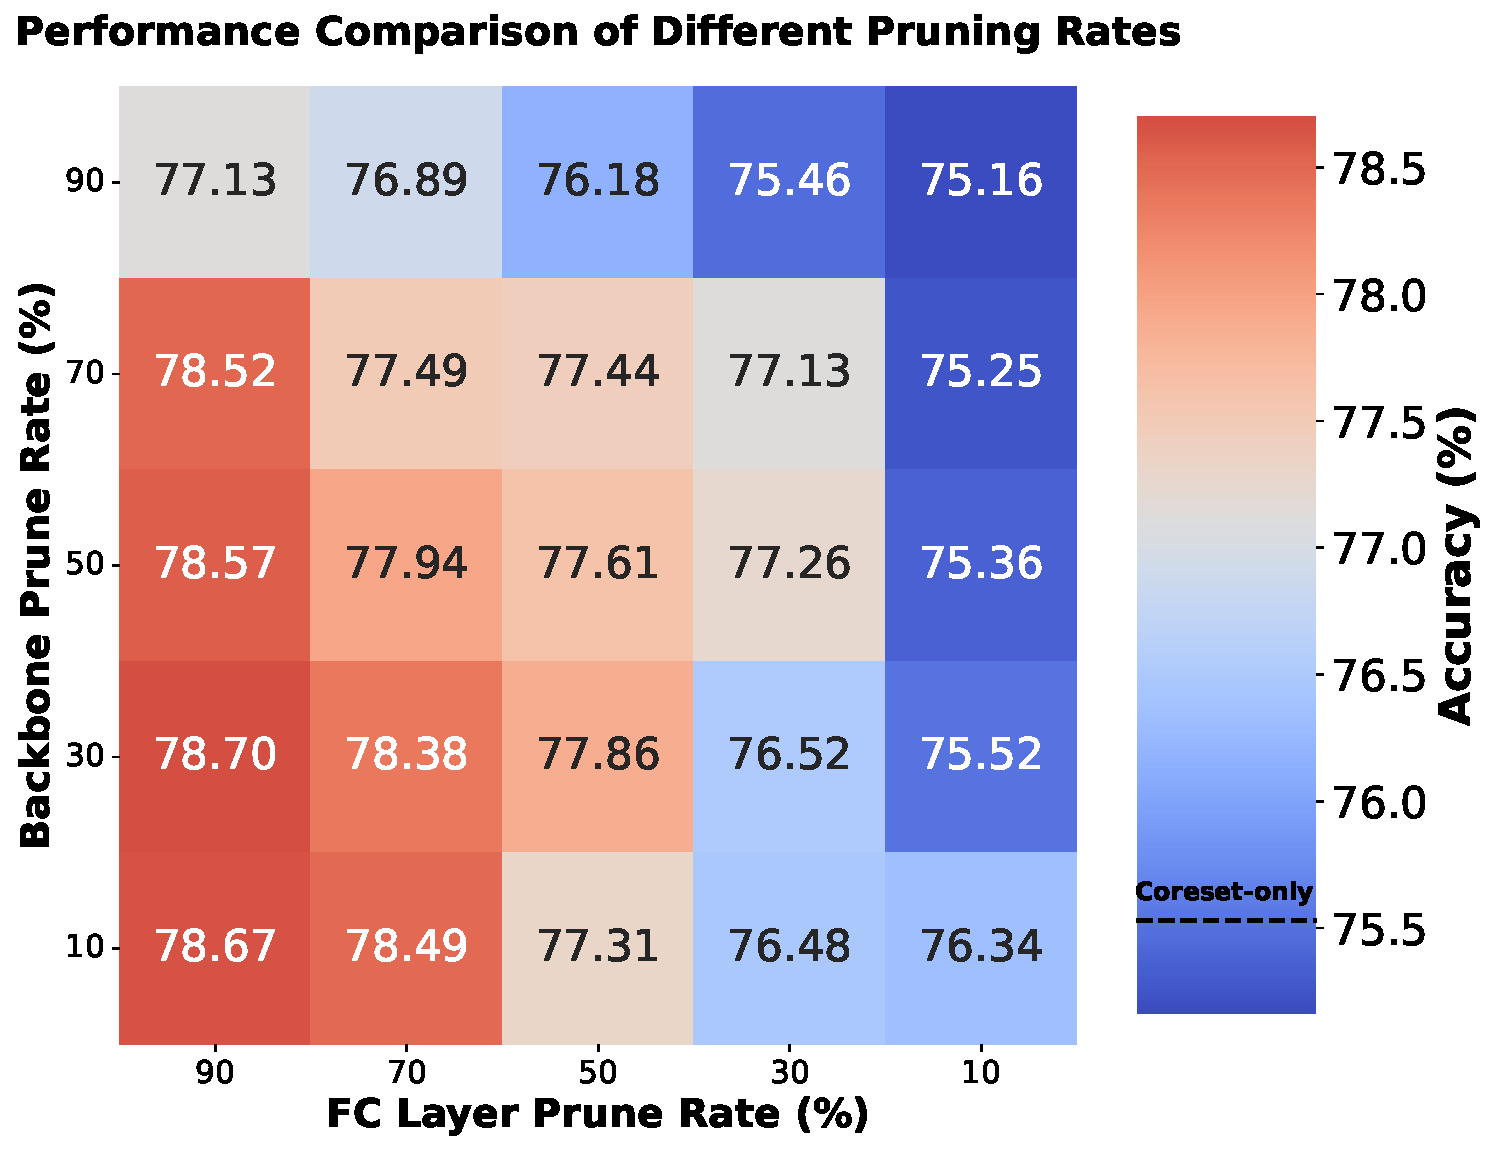
\includegraphics[width=0.8\linewidth]{figs/prune_ablation.pdf}  
   \caption{Performance analysis across different pruning configurations. The x-axis and y-axis represent the pruning rates for FC layers and backbone respectively. Each cell shows the accuracy (\%). The horizontal dashed line indicates the baseline accuracy (75.53\%) from coreset-only. Higher FC layer pruning rates (\(>\)70\%) consistently yield better performance.}  
   \label{fig:prune-ablation}  
\end{figure}


\section{Discussion on state preservation}
\label{appendix:state_preservation}
Our state preservation mechanism fundamentally differs from traditional knowledge distillation (KD). KD transfers knowledge from a teacher to a student model, while our approach preserves the model's historical states during alternating optimization, retaining key information from pruned parameters and reduced datasets to mitigate degradation.

Unlike KD's external teacher-student setup, our mechanism is an internal constraint for co-optimizing weight pruning and coreset selection. Thus, comparisons with KD-based methods that use external models for distillation to enhance post-pruning model performance are inappropriate due to differing objectives and assumptions. By avoiding external models or soft targets, we address unique coreset/pruning challenges without biases, ensuring fair evaluation.
Ablation studies in the main text validate this: applying state preservation to coreset-only or pruning-only scenarios shows no gains, demonstrating it stabilizes joint optimization, not enhances performance like KD.

\section{More result on time efficiency}
\label{appendix:time_efficiency}
To thoroughly evaluate the practical benefits of our framework, we conduct a detailed analysis of its time efficiency in comparison with baseline methods. As shown in Table~\ref{tab:time}, our method with 10\% coreset size achieves comparable accuracy (92.96\%) to the coreset-only method with 15\% data (92.97\%), while requiring significantly less training time (2191s vs 2738s).
\begin{table}[!htbp]  
\footnotesize   
\centering  
\caption{\textbf{Comparison of accuracy and time efficiency.} }   
\label{tab:time}  
\resizebox{\linewidth}{!}{   
\begin{tabular}{@{}cccc@{}}  
\toprule  
\textbf{Settings}  & coreset-only (10\%) & coreset-only (15\%) & \textbf{Ours (10\%)} \\ \midrule  
\textbf{Acc. (\%) ↑}     & 91.13              & 92.97              & \textbf{92.96}      \\
\textbf{Time (sec) ↓} & 2034              & 2738              & \textbf{2191}      \\
\textbf{Params (M) ↓} & 44.5              & 44.5              & \textbf{31.2}      \\ \bottomrule  
\end{tabular}}   
\end{table} 
Moreover, when compared to pruning-only methods using full dataset, ours provides significant speed advantage by using coreset.

\begin{table*}[!htbp] 
    \caption{Comparison of test accuracy (\%) on CIFAR-10 across different training settings. The table is divided into four distinct regions: (1) Standard training ({\color{gray!85}gray}, top-right cell) achieves 85.99\% accuracy with full dataset; (2) Pruning-only training ({\color{orange!85}orange}, top row) shows accuracy under different pruning rates, ranging from -0.14\% to +0.87\%; (3) Coreset-only training ({\color{blue!85}blue}, rightmost column); and (4) Our joint pruning and coreset selection framework ({\color{green!85}green}) demonstrates superior performance with up to +6.12\% improvement over standard training. Values in parentheses indicate differences from the Dense training baseline.} 
    \label{tab:noise_result}
    \centering  
    \resizebox{\textwidth}{!}{  
    \renewcommand{\arraystretch}{1.2}
    \begin{tabular}{lcccccc}  
    \hline  
    & \multicolumn{6}{c}{\textbf{Prune Rate in Joint Weight and Sample Tailoring}} \\ \cline{2-7}  
    \multirow{-2}{*}{\textbf{Subset Fraction}} & 90\% & 70\% & 50\% & 30\% & 10\% & 0\% (Dense) \\ \hline  
    100\% ({\color{orange!85}Pruning-only}) & \cellcolor{orange!15}$85.85_{{\tiny(-0.14)}}$ & \cellcolor{orange!15}$86.12_{{\tiny(+0.13)}}$ & \cellcolor{orange!15}{$86.41_{{\tiny(+0.42)}}$} & \cellcolor{orange!15}{$86.86_{{\tiny(+0.87)}}$} & \cellcolor{orange!15}$86.70_{{\tiny(+0.71)}}$ & \cellcolor{gray!15}$85.99$ (Standard Training) \\ 
    ~20\%~~({\color{green!85}Ours}) & \cellcolor{green!15}$91.08_{{\tiny(+0.75)}}$ & \cellcolor{green!15}$91.86_{{\tiny(+1.53)}}$ & \cellcolor{green!15}{$91.89_{{\tiny(+1.56)}}$} & \cellcolor{green!15}{$92.11_{{\tiny(+1.78)}}$} & \cellcolor{green!15}{$92.04_{{\tiny(+1.71)}}$} & \cellcolor{blue!15}$90.33$ (Coreset-only) \\
    ~10\%~~({\color{green!85}Ours}) & \cellcolor{green!15}$87.82_{{\tiny(+1.01)}}$ & \cellcolor{green!15}$88.37_{{\tiny(+1.56)}}$ & \cellcolor{green!15}{$88.62_{{\tiny(+1.81)}}$} & \cellcolor{green!15}{$88.69_{{\tiny(+1.88)}}$} & \cellcolor{green!15}{$88.64_{{\tiny(+1.83)}}$} & \cellcolor{blue!15}$86.81$ (Coreset-only) \\ 
    ~~5\%~~~({\color{green!85}Ours}) & \cellcolor{green!15}$85.14_{{\tiny(+8.47)}}$ & \cellcolor{green!15}$86.05_{{\tiny(+9.38)}}$ & \cellcolor{green!15}{$86.19_{{\tiny(+9.52)}}$} & \cellcolor{green!15}{$86.45_{{\tiny(+9.78)}}$} & \cellcolor{green!15}{$86.34_{{\tiny(+9.67)}}$} & \cellcolor{blue!15}$76.67$ (Coreset-only) \\ \hline 
    \end{tabular}}  
\end{table*}

\section{Detail results on noisy data}  
\label{appendix:noise_exp}  
To evaluate the robustness of our framework in practical scenarios, we conduct experiments with 20\% noise in training data. As shown in Table~\ref{tab:noise_result}, our method demonstrates remarkable performance even under such noisy conditions. With only 20\% of the training data, our joint framework achieves up to 92.11\% accuracy (+6.12\% improvement over standard training), significantly outperforming both pruning-only (maximum 87.46\%) and coreset-only (90.33\%) approaches. Notably, this superior performance is achieved with substantially reduced computational costs, using both fewer parameters (through pruning) and less training data (through coreset selection). Even when further reducing the data to just 5\%, our method maintains competitive performance (86.45\%), demonstrating its efficiency in handling noisy scenarios with minimal resources. These results highlight that our framework not only enhances model robustness against label noise but also achieves this with significantly lower computational overhead compared to traditional training approaches. 


\begin{table*}[!htbp]   
    \caption{Test accuracy (\%) of our framework using ProbMask as the pruning method. The coreset size is fixed at 10\% of the training set. Values in parentheses indicate differences from the Coreset-only baseline. Red/blue numbers indicate best and runner-up results within each row.}   
    \label{tab:probmask}  
    \centering  
    \resizebox{\linewidth}{!}{  
    \renewcommand{\arraystretch}{1.1}  
    \begin{tabular}{ccccccccc}  
    \hline
    & &  & \multicolumn{5}{c}{\textbf{Prune Rate in Joint Weight and Sample Tailoring}} &  \\ \cline{4-8}  
    \multirow{-2}{*}{\textbf{Pruning Method}} & \multirow{-2}{*}{\textbf{Model}} & \multirow{-2}{*}{\textbf{Dataset}} & 90\% & 70\% & 50\% & 30\% & 10\% & \multirow{-2}{*}{\textbf{Coreset-only}} \\ \hline  
    & & CIFAR-10 & $91.47_{{\tiny(-0.73)}}$ & $92.31_{{\tiny(+0.11)}}$ & {\color{blue}$92.44_{{\tiny(+0.24)}}$} & {\color{red}\textbf{$92.71_{{\tiny(+0.51)}}$}} & {\color{blue}$92.59_{{\tiny(+0.39)}}$} & 92.20 \\   
    & \multirow{-2}{*}{ResNet-18} & CIFAR-100 & $67.74_{{\tiny(-3.23)}}$ & $71.03_{{\tiny(+0.06)}}$ & {\color{blue}$71.56_{{\tiny(+0.59)}}$} & {\color{red}\textbf{$71.93_{{\tiny(+0.96)}}$}} & {\color{blue}$71.87_{{\tiny(+0.90)}}$} & 70.97 \\ \cline{2-9}  
    & & CIFAR-10 & $91.93_{{\tiny(+0.80)}}$ & $92.28_{{\tiny(+1.15)}}$ & {\color{blue}$92.46_{{\tiny(+1.33)}}$} & {\color{red}\textbf{$92.88_{{\tiny(+1.75)}}$}} & {\color{blue}$92.76_{{\tiny(+1.63)}}$} & 91.13 \\   
    \multirow{-4}{*}{ProbMask} & \multirow{-2}{*}{ResNet-101} & CIFAR-100 & $69.18_{{\tiny(+0.39)}}$ & $71.05_{{\tiny(+2.26)}}$ & {\color{blue}$71.74_{{\tiny(+2.95)}}$} & {\color{red}\textbf{$72.19_{{\tiny(+3.40)}}$}} & {\color{blue}$71.96_{{\tiny(+3.17)}}$} & 68.79 \\ \hline   
    \end{tabular}}  
\end{table*}

\begin{table*}[!t]   
    \caption{Test accuracy (\%) of our framework using ProbMask as the pruning method. Each entry shows the test accuracy with the relative improvement over coreset-only baseline in subscript. The coreset size is fixed at 10\% of the training set. Red/blue numbers indicate best and runner-up results within each row.}   
    \label{tab:other_coreset_method}  
    \centering  
    \resizebox{\linewidth}{!}{  
    \renewcommand{\arraystretch}{1.1}  
    \begin{tabular}{cccccccc}  
    \hline
    &  & \multicolumn{5}{c}{\textbf{Prune Rate in Joint Weight and Sample Tailoring}} &  \\ \cline{3-7}  
    \multirow{-2}{*}{\textbf{Coreset Methods}} & \multirow{-2}{*}{\textbf{Model}} & 90\% & 70\% & 50\% & 30\% & 10\% & \multirow{-2}{*}{\textbf{Coreset-only}} \\ \midrule  
    & ResNet-18 & $90.87_{{\tiny(+1.54)}}$ & $91.41_{{\tiny(+2.08)}}$ & {\color{blue}$91.63_{{\tiny(+2.30)}}$} & {\color{red}\textbf{$91.77_{{\tiny(+2.44)}}$}} & {\color{blue}$91.75_{{\tiny(+2.42)}}$} & 89.33 \\   
    \multirow{-2}{*}{CRAIG} & ResNet-101 & $91.03_{{\tiny(+5.76)}}$ & $91.66_{{\tiny(+6.39)}}$ & {\color{blue}$91.80_{{\tiny(+6.53)}}$} & {\color{red}\textbf{$91.82_{{\tiny(+6.55)}}$}} & {\color{blue}$91.71_{{\tiny(+6.44)}}$} & 85.27 \\ \hline  
    & ResNet-18 & $91.42_{{\tiny(-0.83)}}$ & $92.50_{{\tiny(+0.25)}}$ & {\color{blue}$92.62_{{\tiny(+0.37)}}$} & {\color{red}\textbf{$92.85_{{\tiny(+0.60)}}$}} & {\color{blue}$92.79_{{\tiny(+0.54)}}$} & 92.25 \\
    \multirow{-2}{*}{Glister} & ResNet-101 & $91.82_{{\tiny(+0.36)}}$ & $92.61_{{\tiny(+1.15)}}$ & {\color{blue}$92.95_{{\tiny(+1.49)}}$} & {\color{red}\textbf{$93.12_{{\tiny(+1.66)}}$}} & {\color{blue}$93.03_{{\tiny(+1.57)}}$} & 91.46 \\ \hline  
    & ResNet-18 & $91.12_{{\tiny(+0.33)}}$ & $91.35_{{\tiny(+0.56)}}$ & {\color{blue}$91.58_{{\tiny(+0.79)}}$} & {\color{red}\textbf{$91.67_{{\tiny(+0.88)}}$}} & {\color{blue}$91.55_{{\tiny(+0.76)}}$} & 90.79 \\   
    \multirow{-2}{*}{Moderate} & ResNet-101 & $91.24_{{\tiny(+3.07)}}$ & $91.39_{{\tiny(+3.22)}}$ & {\color{blue}$91.65_{{\tiny(+3.48)}}$} & {\color{red}\textbf{$91.88_{{\tiny(+3.71)}}$}} & {\color{blue}$91.74_{{\tiny(+3.57)}}$} & 88.17 \\ \hline  
    \end{tabular}}  
\end{table*}

\section{Generalization}
\label{appendix:using_other_method}
As emphasized in our main text, a key advantage of our proposed framework lies in its flexibility and generalizability. Our framework is designed to accommodate a wide range of alternative approaches. This section demonstrates this generalizability through comprehensive experiments with different pruning algorithms and coreset selection methods. The following subsections present experimental results that validate our framework's compatibility with various methods, while maintaining consistent performance improvements.

\subsection{Generalization on pruning method}
To demonstrate the generality of our framework, we evaluate its performance using ProbMask~\cite{zhou2022probabilistic} as an alternative pruning method. As shown in Table~\ref{tab:probmask}, our framework maintains its effectiveness across different network architectures (ResNet-18 and ResNet-101) and datasets (CIFAR-10 and CIFAR-100). With ResNet-18, we achieve improvements of up to +0.51\% and +0.96\% over the coreset-only baseline on CIFAR-10 and CIFAR-100, respectively. The benefits become more pronounced with ResNet-101, where we observe larger gains of up to +1.75\% on CIFAR-10 and +3.40\% on CIFAR-100. Notably, the optimal performance consistently occurs at moderate pruning rates (around 30\%), regardless of the model architecture or dataset. These results suggest that our framework's ability to jointly optimize network structure and training data is not tied to specific pruning methods, demonstrating its potential as a general approach for efficient deep learning.

\subsection{Generalization on coreset selection method}
To further validate the versatility of SWaST, we evaluate its performance with different coreset selection methods, including CRAIG~\cite{mirzasoleiman2020coresets}, Glister~\cite{killamsetty2021glister}, and Moderate~\cite{xia2022moderate}. As shown in Table~\ref{tab:other_coreset_method}, our framework consistently improves upon the coreset-only baselines across all methods and architectures. With CRAIG, we achieve substantial improvements of up to +2.44\% and +6.55\% on ResNet-18 and ResNet-101, respectively. Similar patterns are observed with GLISTER (up to +0.60\% and +1.66\%) and Moderate (up to +0.88\% and +3.71\%). Notably, across all coreset methods, the optimal performance is consistently achieved at 30\% pruning rate, suggesting a robust sweet spot for the pruning-coreset trade-off. These results demonstrate that our framework's effectiveness is not limited to specific coreset selection algorithms, but rather provides a general approach for combining network pruning with data selection, regardless of the underlying coreset method.

\section{Limitations}
\label{appendix:limitation}
While our framework demonstrates promising results in joint optimization of network structure and training data, there are certain limitations in practical acceleration that warrant discussion. Although our approach theoretically enables multiplicative speedup - combining the acceleration from weight pruning ($a\times$) and coreset selection ($b\times$) - achieving the full $a \times b$ acceleration in practice remains challenging. This gap between theoretical and practical speedup primarily stems from the current limitations in implementing efficient sparse computation.
The main challenge lies in translating theoretical sparsity into practical acceleration through weight pruning. Modern deep learning frameworks and hardware are often optimized for dense computation, making it difficult to fully capitalize on the potential benefits of sparse networks without substantial engineering efforts. These efforts would include developing specialized sparse computation kernels, implementing efficient model instantiation mechanisms, and optimizing hardware-specific operations.

